\chapter{Designing Web Application Platform}
\label{chapter4}
\thispagestyle{plain}
In this chapter we will go through necessary phases required to develop a software solution. This chapter is entirely focused on the design and modelling of the software solution, regardless of the underlying programming languages or development platform of choice. We use UML \footnote{The Unified Modeling Language(UML)} in order to make a model of our proposed solution.
UML is a general-purpose, developmental, modeling language in the field of software engineering that is intended to provide a standard way to visualize the design of a system. In addition we need to make model of business processes and main activities, we will see BPMN \footnote{Business Process Model and Notation(BPMN)} diagrams throughout this chapter. 

\section{Software Modelling}
\subsection{Use Case Diagram}
UML use case diagrams describe relevant functionalities of the business process, the users/actors involved in execution of the business process, and the assignment of functionalities to users/actors.

Use case diagram visualizes functional requirements of the system which were previously defined in requirement analysis section of chapter one. As it is evident in figure \ref{fig:uml_usecase_model},  some use cases are linked only to one actor, while others involve two or more actors based on nature of the task.

Figure \ref{fig:uml_usecase_model} illustrates use case diagram for our digital booking platform. Main actors of the system are "Platform Manager", "Property Owner" and "Guest". These actors are connected to their respective functionalities which are indicated as oval shaped figures in the use case diagram.

\begin{figure} 
\centering
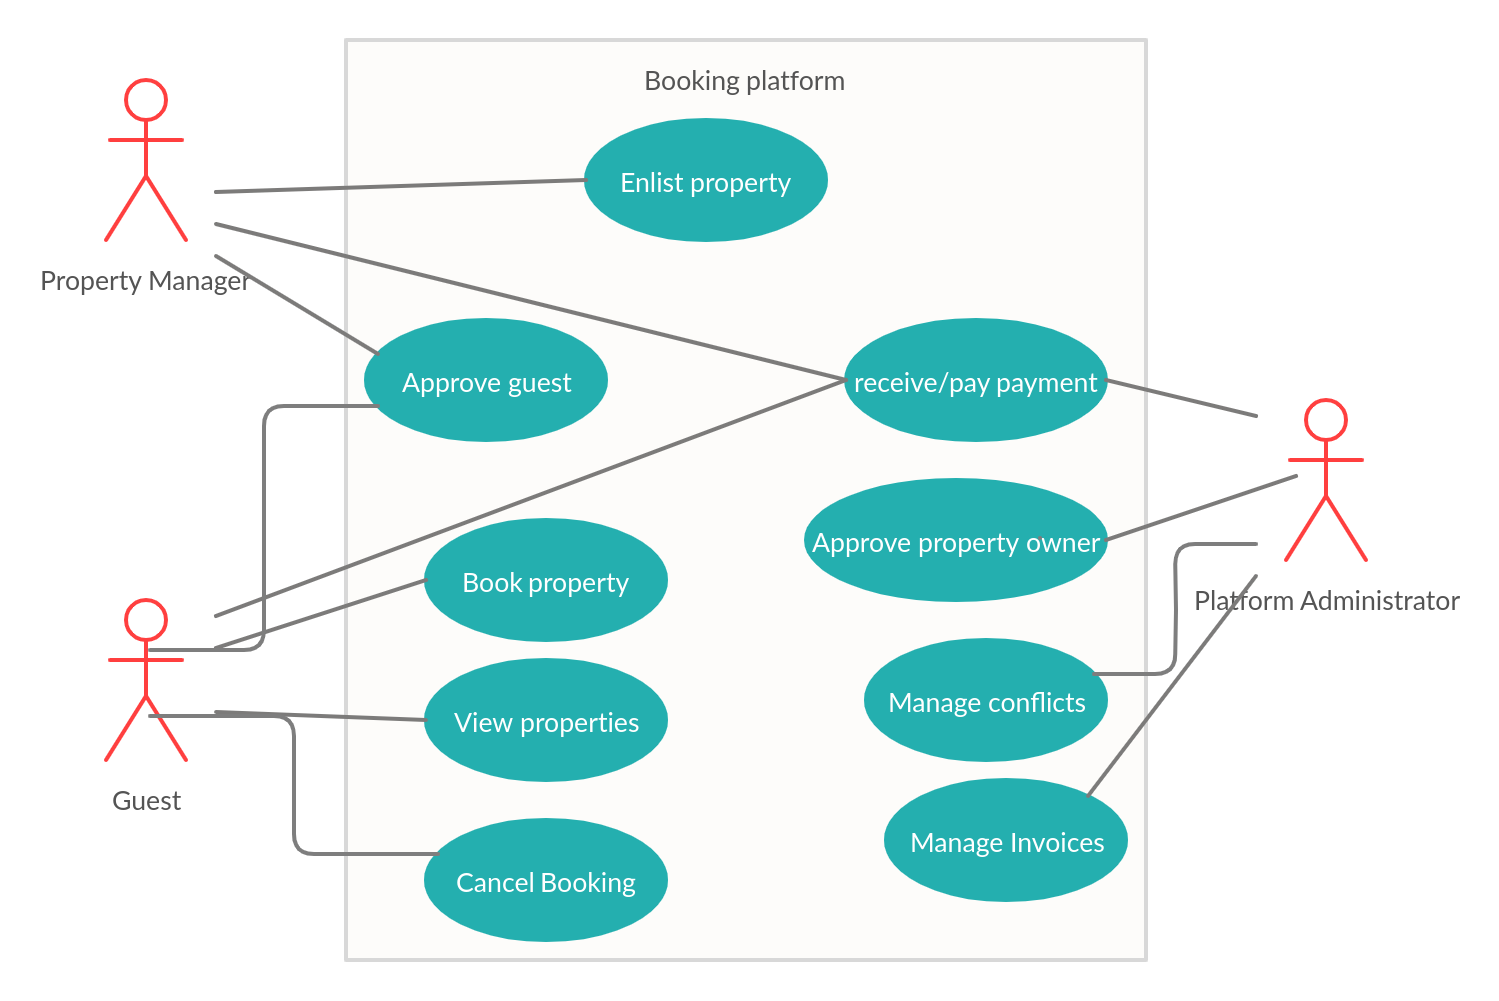
\includegraphics[width=12cm]{pictures/UML_usecase_diagram.png}
\caption{Use case Diagram}
Figure illustrating Use case diagram, part of UML modelling diagrams.
\label{fig:uml_usecase_model}
\end{figure}

\subsection{Class Diagram}
UML class diagrams report the schema of the underlying information model. We need class diagram in order to describe the structure of our system by showing the system's classes, their attributes, operations (or methods), and the relationships among objects.
Figure \ref{fig:uml_class_model} illustrates our digital booking platform classes and the relationship among objects. As the figure \ref{fig:uml_class_model} illustrates, there are four essential classes identified for our system namely "Guest", "Platform Administrator", "Property Owner" and "Booking".
In addition figure \ref{fig:uml_class_model} also shows association relationships among identified classes which are shown by the numbers on both ends of the association relationship. These associations are essential for designing database tables and placement of foreign keys later on. 
One of the important aspects of modelling UML class diagram is the fact that, class diagram provides a solid foundation about the structure of classes which later on we will use when in the implement ion of our system.

\begin{figure} 
\centering
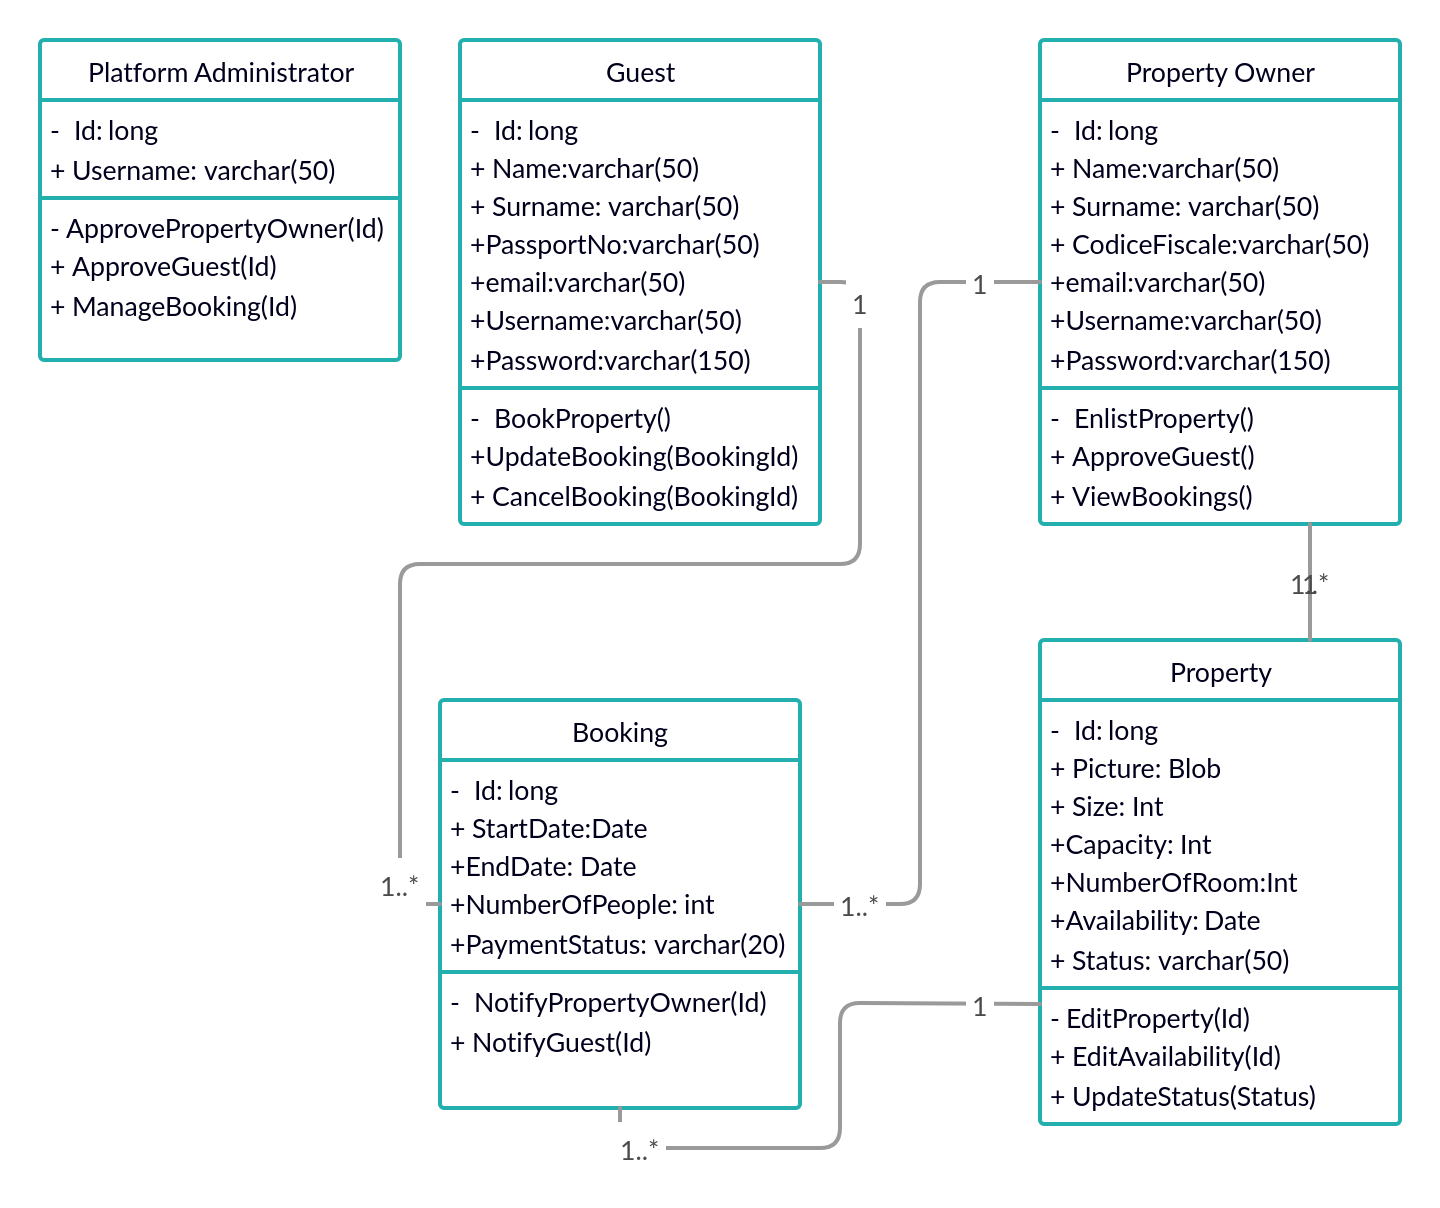
\includegraphics[width=12cm]{pictures/UML_class_diagram.png}
\caption{UML Class Diagram}
Figure illustrating UML class diagram, part of UML modelling diagrams.
\label{fig:uml_class_model}
\end{figure}
 
\subsection{Business Process Modeling Diagram}
After identifying the main actors and functionalities of the system, we need to further examine the flow of the business processes which occur inside the system. For this purpose we use Business Process Modelling in particular BPMN \footnote{business Process Model and Notation(BPMN)}.
BPMN is a widely used standard for process modeling. In BPMN, activities are represented as round rectangles, Control nodes (called gateways) are represented using diamond shapes finally Activities and control nodes are connected by means of arcs (called flows) that determine the order in which the process is executed.
Figure \ref{fig:bpmn_notion_pic} shows various types of gateways used in our business process diagrams.

\begin{figure} 
\centering
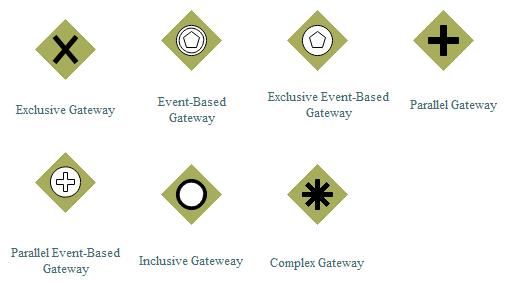
\includegraphics[width=14cm]{pictures/BPMN_NOTION2.png}
\caption{BPMN gateways}
Figure illustrating BPMN gateways.
\label{fig:bpmn_notion_pic}
\end{figure}


Figure \ref{fig:bpm_guest_model} illustrates business process of booking by Guest. 
In this process we use \textit{exclusive gateway} which evaluates the state of the business process and, based on the condition, breaks the flow into one of the two or more mutually exclusive paths.
In addition we can see parallel tasks which execute concurrently, as shown in figure \ref{fig:bpm_guest_model} "Check Availability" and "Check approval by Owner" tasks are executed concurrently in the booking process.
Final point which we need to address is usage of time based events. A clock icon represents the timer event, we used this technique in order to indicate the payment is bound to a time limit in this case 60 minutes, in this way guest must finalize the booking by doing the "payment transaction" task otherwise the booking process ends. 

\begin{figure} 
\centering
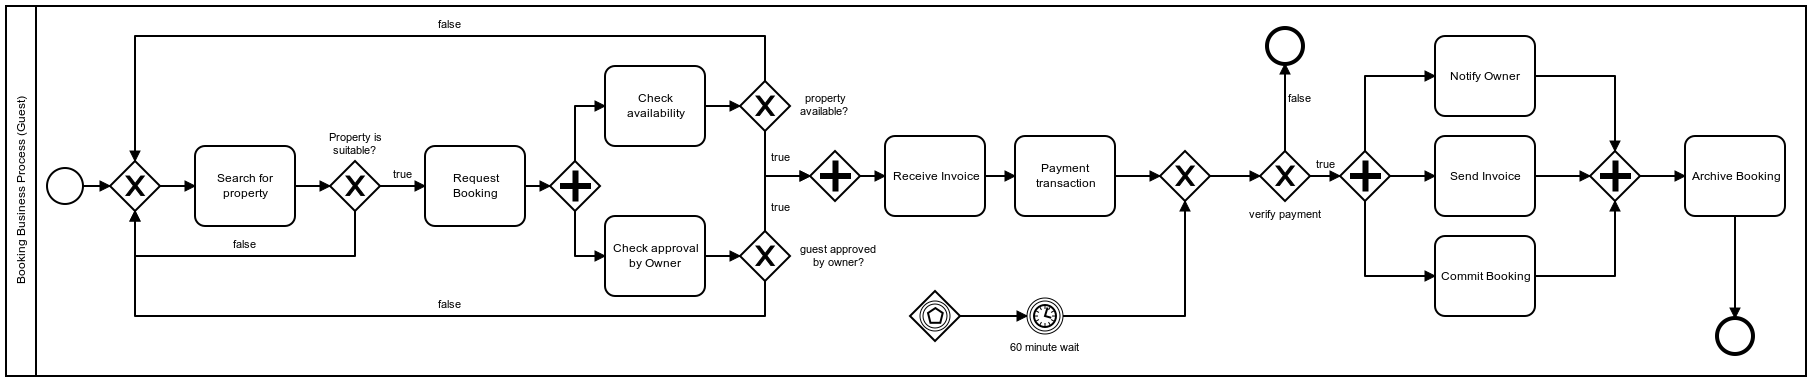
\includegraphics[width=14cm]{pictures/BPMN_guest.png}
\caption{BPMN guest Diagram}
Figure illustrating BPMN guest Diagram.
\label{fig:bpm_guest_model}
\end{figure}


%The diagram indicates the logical flow of the business process of which we need to incorporate in our system. 
%BPMN allows us to use

 Figure \ref{fig:bpm_owner_model} illustrates business process of booking from perspective of property owner. Property owner firstly registers to the platform, the platform then validates property owner and property owner is given permission to enlist his/her property for booking. After enlisting the property the business process stops until there is a \textit{signal} indicating a request for booking, the property owner has a choice of approving or rejecting the request. Upon accepting the request "Receive payment" and "Archive transaction" processes will execute simultaneously and finally the business process ends. 

\begin{figure} 
\centering
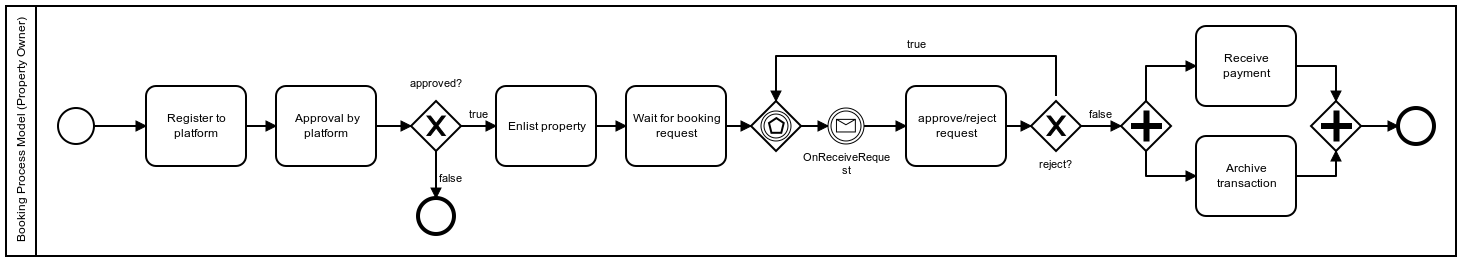
\includegraphics[width=14cm]{pictures/BPMN_property_owner.png}
\caption{BPMN property owner Diagram}
Figure illustrating BPMN property owner Diagram.
\label{fig:bpm_owner_model}
\end{figure}


Figure \ref{fig:bpm_platform_owner_model} illustrates the process of "Managing dispute" between "Property owner" and "Guest" from perspective of platform administrator. The process begins by simultaneous validation of Property Owner's clam and Guest's claim. Once this is done, one of the claim's is chosen as a "valid" claim. If we consider Owner claim as the valid claim, the status of payment by the "Guest" is evaluated, and the security deposit of the Guest is collected in case the Guest has already paid the security deposit. Then the guest is notified and the process ends. On the other hand if the guest's claim turns out to be valid, guest will receive a refund from the platform and property owner will receive a warning.

\begin{figure} 
\centering
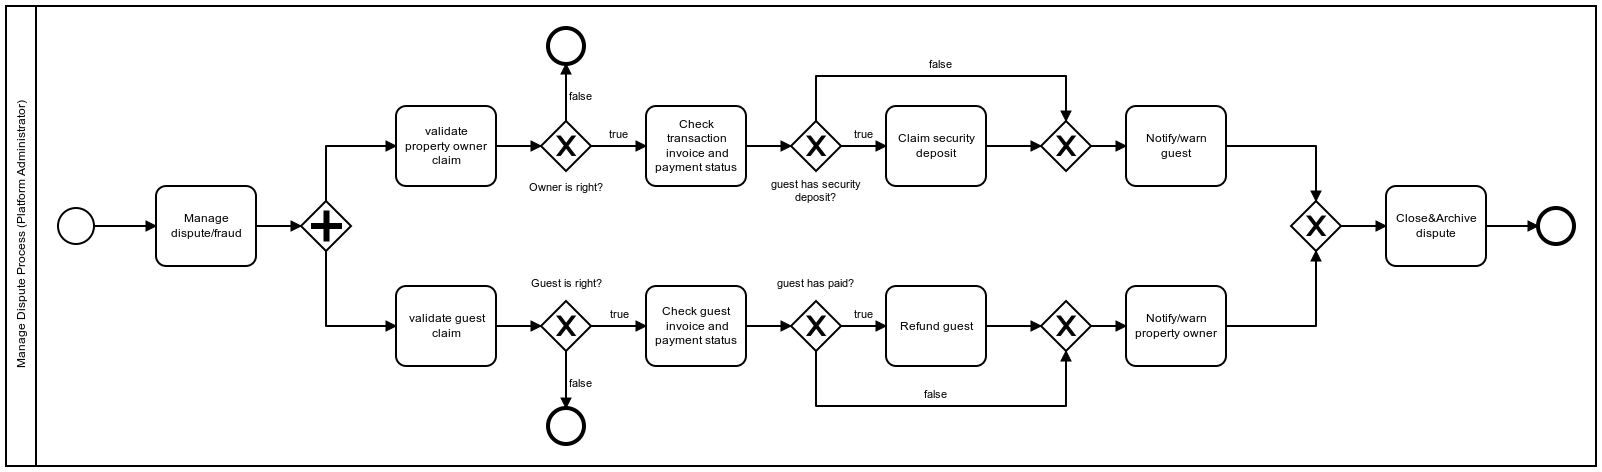
\includegraphics[width=14cm]{pictures/BPMN_platform_owner.png}
\caption{BPMN platform owner Diagram}
Figure illustrating BPMN platform owner Diagram.
\label{fig:bpm_platform_owner_model}
\end{figure}

Figure \ref{fig:bpm_guest_update_model} illustrate guest update/cancel booking business process. As it is evident from the diagram, firstly we must check for the status of booking in case the booking is not locked the process continues and the guest is given options to either change date/duration of stay, edit number of guests or simply cancel the booking altogether. Upon choice of edit by guest, the platform checks for availability of the property in the specified period, in case property is available the change made by Guest is confirmed and the process continues by sending invoice and wait for payment. In case the Guest decides not to commit payment, the timer will continue the process and as a result verify payment check returns false and consequently the process ends.

\begin{figure} 
\centering
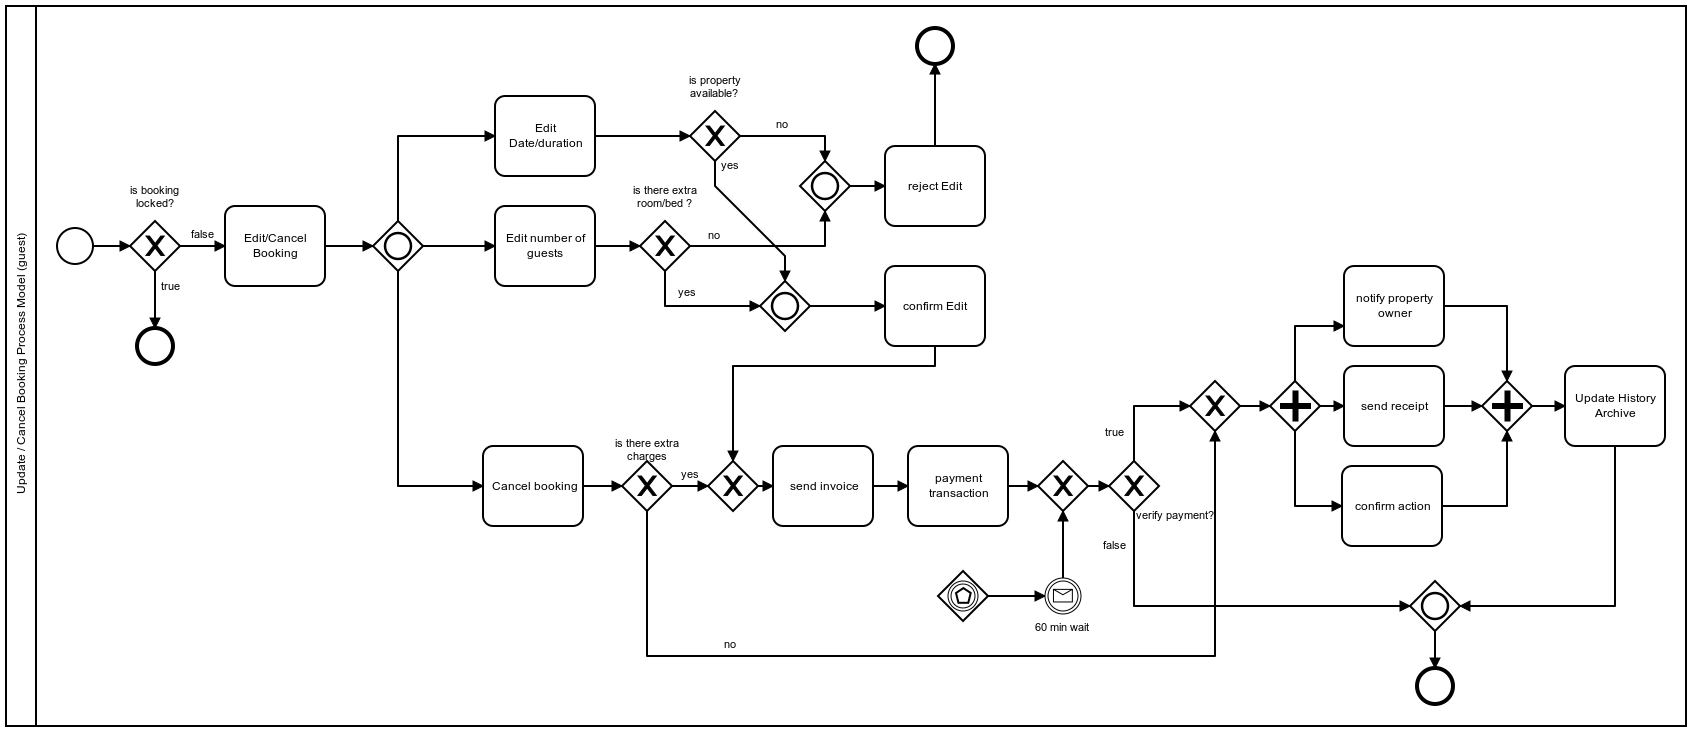
\includegraphics[width=14cm]{pictures/BPMN_guest_update.png}
\caption{BPMN guest update booking Diagram}
Figure illustrating BPMN guest update booking Diagram.
\label{fig:bpm_guest_update_model}
\end{figure}


Now that we have seen the main structure of our system throughout UML use case diagram, UML class diagram and BPMN business process diagrams, we arrive at design of database structure for our digital booking platform project. We complete this chapter by representing our database structure represented in Figure \ref{fig:database_diagram}. As evident from the picture, the tables are similar in structure to the class diagram represented in figure \ref{fig:uml_class_model}. In addition the choice of primary and foreign keys is a direct result of the UML class diagram relationships.

\begin{figure} 
\centering
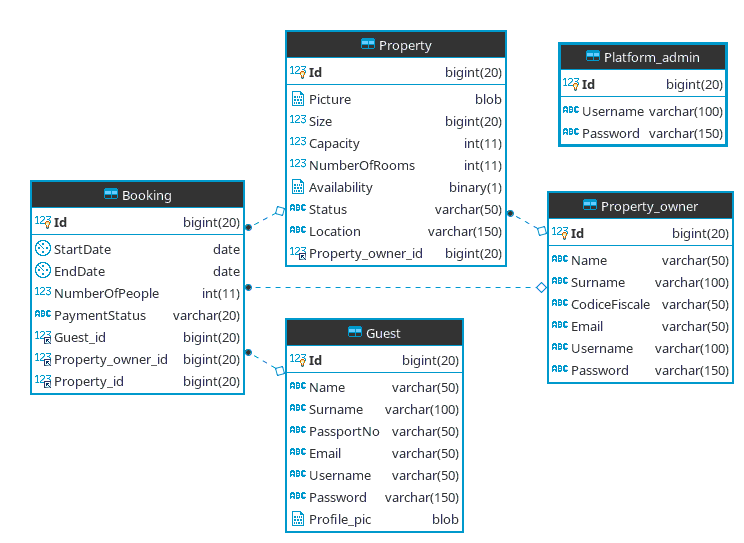
\includegraphics[width=14cm]{pictures/database_diagram.png}
\caption{Database structure of digital booking platform}
Figure illustrating main tables as well as relationship among tables through usage of foreign keys.
\label{fig:database_diagram}
\end{figure}



%\section{Hardware }

